%
% 07_stetige_kurven.tex -- Einfuhrung in den Satz von Jordan fuer stetige Kurven
%
% (c) 2026 Dominik Castelberg, Ostschweizer Fachhochschule
%
% !TEX root = ../../buch.tex
% !TEX encoding = UTF-8
%

\section{Der Fall stetiger Kurven
\label{jordan:section:stetige_kurven}}
\kopfrechts{Der Fall stetiger Kurven}

Mit der Nutzung der Umlaufzahl als zentrales Werkzeug für den Beweis des Satzes von Jordan haben wir es sehr weit gebracht.
Die Fälle, welche wir bisher behandelt haben, decken einen Grossteil der in der Praxis auftretenden Kurven ab, und die erarbeiteten Werkzeuge sind bereits jetzt sehr mächtig.

Stetige Kurven bieten jedoch ein ganz anderes Kaliber an Komplexität: Sie können sehr wild und an keinem Punkt differenzierbar sein, und die Tangentenrichtung ist nicht wohldefiniert.
Beispiele für stetige Kurven beinhalten:

\begin{itemize}
    \item \textbf{Fraktale Jordan-Kurven:} Die Koch-Schneeflocke, der Rand der Mandelbrot-Menge und das Sierpinski-Dreieck sind klassische Beispiele für stetige Jordan-Kurven und haben eine Hausdorff-Dimension von $>1$. Solche Kurven sind lokal beliebig komplex.
    \item \textbf{Die Weierstrass-Funktion-basierte Kurve:} Der Graph der Weierstrass-Funktion 
    \[
    f(x) = \sum_{n=0}^{\infty} a^n \cos(b^n \pi x)
    \]
    für $0 < a < 1$ und ungerades $b$, welcher durch das Schliessen mit einem Kreisbogen zu einer Jordan-Kurve ergänzt werden kann, ist stetig, aber an keinem Punkt auf einem Teilbogen differenzierbar.
    \item \textbf{Kurven mit positivem Flächenmass:} Osgood konstruierte 1903 eine Jordan-Kurve mit positivem Lebesgue-Mass.
\end{itemize}

\begin{figure}
    \centering
    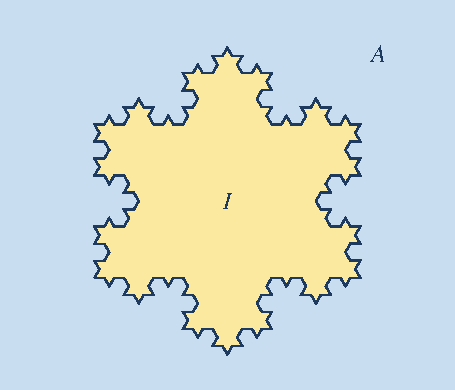
\includegraphics{papers/jordan/images/koch_schneeflocke.pdf}
    \caption{Koch-Schneeflocke als Beispiel für ein Fraktal, dargestellt mit Iterationstiefe 3.}
\end{figure}

Mit der Erweiterung von stückweise $C^1$-Jordan-Kurven auf stetige Jordan-Kurven stehen wir also vor einer riesigen Herausforderung: Der Tangentenvektor ist nicht mehr wohldefiniert und da die Kurven nicht differenzierbar sind, können wir keine Kurvenintegrale $\oint_{\gamma}$, wie wir sie bisher verstanden haben, berechnen.
Diese Verluste sind für unsere bisherige Argumentation fatal, da wir hiermit zahlreiche Werkzeuge verlieren, welche wir ohne ein grundsätzliches Umdenken nicht ersetzen können:

\begin{enumerate}
    \item Da wir weder Tangenten noch Normalen haben, können wir keine tubulare Umgebung mehr definieren.
    \item Mit dem Verlust des Kurvenintegrals $\oint_{\gamma}$ verlieren wir die Definition der Umlaufzahl.
    \item Als Konsequenz verlieren sowohl den Hopfschen Umlaufsatz als auch den Gauss-Bonnet-Satz.
\end{enumerate}

Die Werkzeuge der komplexen Algebra stossen hier an ihre Grenzen.
Die gute Nachricht ist, jedoch, dass noch nicht alles verloren ist. 
Manchmal muss man einfach verworfene Werkzeuge wieder hervorholen, um neue Probleme mit alten Mitteln zu lösen.

\subsection{Polygonale Approximation stetiger Jordan-Kurven}

Aufmerksame Leser haben sich vielleicht gefragt, warum wir in einem Buch über Analysis und Algebra in diesem Kapitel so viel Zeit mit geometrischen Argumenten und konstruktiven Beweisen für Polygone verbracht haben.
Die Antwort ist einfach: Polygone sind die einfachsten geometrischen Objekte, die wir verwenden können, um beliebige stetige Kurven beliebig genau zu approximieren.

\begin{figure}
    \centering
    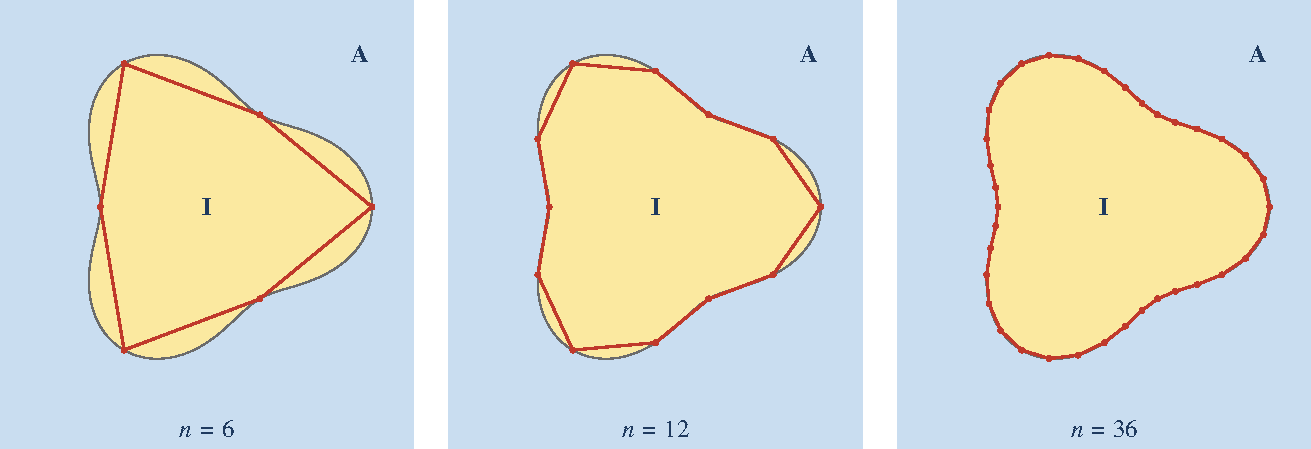
\includegraphics{papers/jordan/images/polygonale_approximation.pdf}
    \caption{Polygonale Approximation einer stetigen Kurve.}
\end{figure}

\begin{satz}[Polygonale Approximation stetiger Jordan-Kurven\label{jordan:satz:polygonale_approximation_stetiger_jordan_kurven}]
    Sei $\gamma \subset \mathbb{R}^2$ eine stetige Jordan-Kurve. Dann existiert zu jedem $\delta > 0$ ein einfaches Polygon $P_{\delta}$ mit folgenden Eigenschaften:
    \begin{enumerate}
        \item Als einfaches Polygon ist $P_{\delta}$ eine Jordan-Kurve.
        \item Der Hausdorff-Abstand $d_{\mathcal{H}}(\gamma, P_{\delta}) < \delta$.
        \item $P_{\delta}$ besitzt eine Parametrisierung $p_{\delta} : S^1 \to \mathbb{R}^2$ mit $\sup_{t} \left\| \gamma(t) - p_{\delta}(t) \right\| < \delta$.
    \end{enumerate}
\end{satz}



Zu beachten ist hierbei, dass mit ungenügender Granularität der Approximation das entstehende Polygon sich selbst schneiden kann, auch wenn die approximierte Kurve eine valide Jordan-Kurve ist.
Eine stetige Kurve kann im Kleinen beliebig verwinkelt sein, und dieses Problem verschwindet nicht alleine dadurch, dass man die Punkte dichter wählt.
Wir benötigen daher zwei Schwellwerte:

\begin{itemize}
    \item $\eta$ sorgt dafür, dass das Polygon der zu approximierenden Kurve nahe bleibt.
    \item $\varepsilon$ sorgt dafür, dass Selbstschnitte nur lokal auftreten können.
\end{itemize}

\subsubsection{Die Feinheit von $\eta$}

Da $\gamma$ auf dem kompakten Kreis $S^1$ definiert und stetig ist, ist sie gleichmässig stetig.
Daher gibt es eine einzige Schranke, die überall auf der Kurve gleichzeitig funktioniert.
Zu der Genauigkeit $\delta$ finden wir also ein $\eta > 0$ mit
\[
    |t - t'| < \eta \rightarrow \|\gamma(t) - \gamma(t')\| < \frac{\delta}{4}
\]
Dabei misst $|t - t'|$ den Abstand der Parameterwerte auf dem Kreis $S^1$. 
Die Zahl $\eta$ ist nicht eindeutig, da jedes kleinere $\eta$ die Bedingung ebenfalls erfüllt.
Unterteilen wir $S^1$ so, dass benachbarte Parameterwerte weniger als $\eta$ auseinanderliegen, überbrückt jede Kante des Polygons nur ein Stück der Kurve.
Jeder Punkt der Kante liegt also höchstens $\delta/4$ vom Anfangspunkt der Kante entfernt, genauso wie jeder Punkt des zugehörigen Kurvenstücks.
Insgesamt weicht das Polygon an jeder Stelle um weniger als $\delta / 2$ von der Kurve ab.

\subsubsection{Der Mindestabstand $\varepsilon$}

Der zweite Schwellwert $\varepsilon$ nutzt die Einfachheit der Kurve $\gamma$ aus.
Beim Betrachten sämtlicher Paare von Parameterwerten $(t, t')$, die mindestens $\eta$ auseinanderliegen, stellen wir fest, dass jedes Paar verschiedene zugehörige Punkte auf $\gamma$ liefert, und somit einen positiven Abstand hat.
Diese Paare bilden dabei eine kompakte Menge, weshalb der Abstand zwischen den Punkten auf $\gamma$ einen positiven Mindestabstand $\varepsilon$ hat.

\[
  |t - t'| \ge \eta \rightarrow \|\gamma(t) - \gamma(t')\| \ge \varepsilon .
\]

Abschnitte der Kurve, die im Durchlauf weit auseinanderliegen, kommen sich also in der Ebene nie näher als $\varepsilon$.

\subsubsection{Auschluss von Selbstschnitten unter nicht-benachbarten Kanten}

Wir wählen nun die Unterteilung von $\gamma$ fein genug, damit jede Kante des Polygons kürzer als $\varepsilon / 3$ ist.
Angenommen, zwei Kanten schneiden sich in einem Punkt: Da beide Kanten kurz sind, liegen ihre Anfangspunkte dann jeweils weniger als $\varepsilon / 3$ vom Schnittpunkt entfernt, also weniger als $2 \varepsilon / 3$ voneinander.

Gemäss der Definition von $\varepsilon$ ist das nur möglich, wenn ihre Parameterwerte weniger als $\eta$ auseinanderliegen.

\[
  e_i \cap e_j \neq \emptyset \rightarrow |t_i - t_j| < \eta .
\]

Wir können also daraus schliessen, dass Schnitte nur zwischen Kanten auftreten, die auf der Kurve nahe beieinander liegen.

\subsubsection{Bereinigen des Polygons von Schleifen}

Im Falle eines Schnitts bildet das Polygon zwischen den betroffenen Kanten eine Schleife.
Indem wir am Schnittpunkt direkt zur späteren Kante übergehen, können wir die Schleife entfernen und das Polygon wieder zu einer validen Jordan-Kurve machen.
Da das Polygon nur endlich viele Kanten hat, ist nach endlich vielen Schritten keine Schleife mehr übrig.

Wir müssen jedoch sicherstellen, dass wir die Kurve nicht zu stark verändern und die Nähe zur originalen Kurve $\gamma$ erhalten bleibt.
Jede entfernte Schleife gehört zu einem kurzen Parameterstück, das höchstens $2 \eta$ lang ist.
Dieses Parameterstück bewegt die Kurve höchstens $\delta / 2$ von der originalen Kurve weg, und der Schnittpunkt liegt weniger als $\varepsilon / 3$ vom Kurvenstück entfernt.
Wegen $\varepsilon < \delta$ ergibt sich also überall

\[
    \sup_{t \in S^1} \|\gamma(t) - p_\delta(t)\| < \frac{\delta}{2} + \frac{\varepsilon}{3} < \delta.
\]

Hiermit haben wir eine Approximation der stetigen Kurve $\gamma$ durch ein einfaches Polygon $p_\delta$ konstruiert, das beliebig nahe an $\gamma$ liegt und alle in Satz \ref{jordan:satz:polygonale_approximation_stetiger_jordan_kurven} erwähnten Eigenschaften erfüllt.

\subsection{Beweis des Satzes von Jordan für stetige Kurven}

Nach der Approximation der stetigen Kurve $\gamma$ durch ein einfaches Polygon $p_\delta$ können wir die in Sektion \ref{jordan:section:einfache_polygone} erarbeiteten Werkzeuge verwenden, um die Gültigkeit des Satzes von Jordan für $p_\delta$ zu zeigen.

Wenn wir jedoch ehrlich sind, haben wir den Satz von Jordan für stetige Kurven nicht wirklich bewiesen, sondern nur gezeigt, dass er für ein beliebig ähnliches einfaches Polygon gilt.
Dieser Makel macht diesen Beweis unvollständig und für viele Leser unbefriedigend.

Ein ähnliches Gefühl über damalig existierende Beweisansätze hatte wohl auch James W. Alexander, welcher mit seinem Paper \cite{jordan:Alexander1922} einen rigorosen und verallgemeinerten Beweis des Jordan-Brouwer Zerlegungssatzes, und damit auch des Satzes von Jordan, veröffentlichte und dabei die Entwicklung des Forschungsgebiets der algebraischen Topologie massgeblich prägte.